\chapter{Аналитический раздел}
Поисковая система состоит из двух основных компонентов: поискового робота, осуществляющего сбор данных в сети Интернет, и поисковика, осуществляющего поиск по индексу релевантных запросу документов и их ранжирование.

Поисковой робот (рис. \ref{fig:collecting-a0}) находит страницы в сети, используя ссылки с уже проиндексированных страниц. Начальный набор страниц задаётся пользователем, как и конфигурация робота (глубина обхода и другие).

\begin{figure}[h]
  \centering
  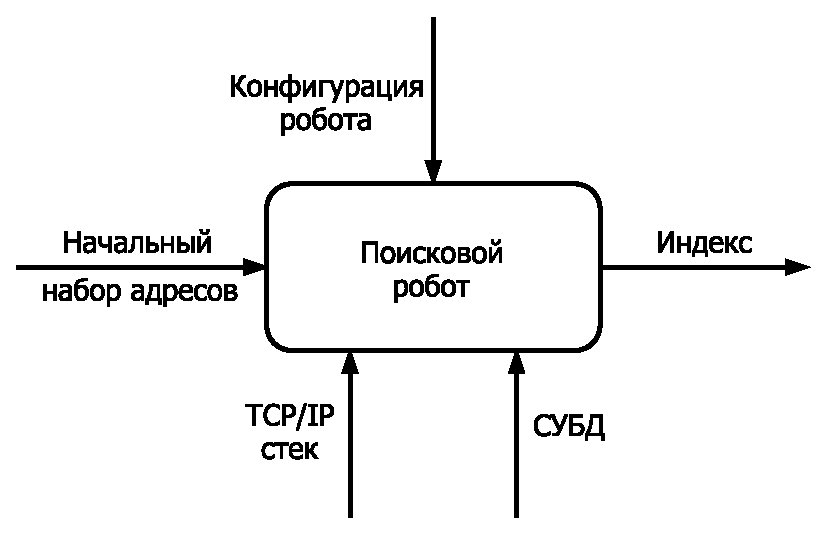
\includegraphics[width=.7\linewidth]{collecting-a0.pdf}
  \caption{IDEF0-A0 поискового робота.}
  \label{fig:collecting-a0}
\end{figure}

\begin{figure}[h]
  \centering
  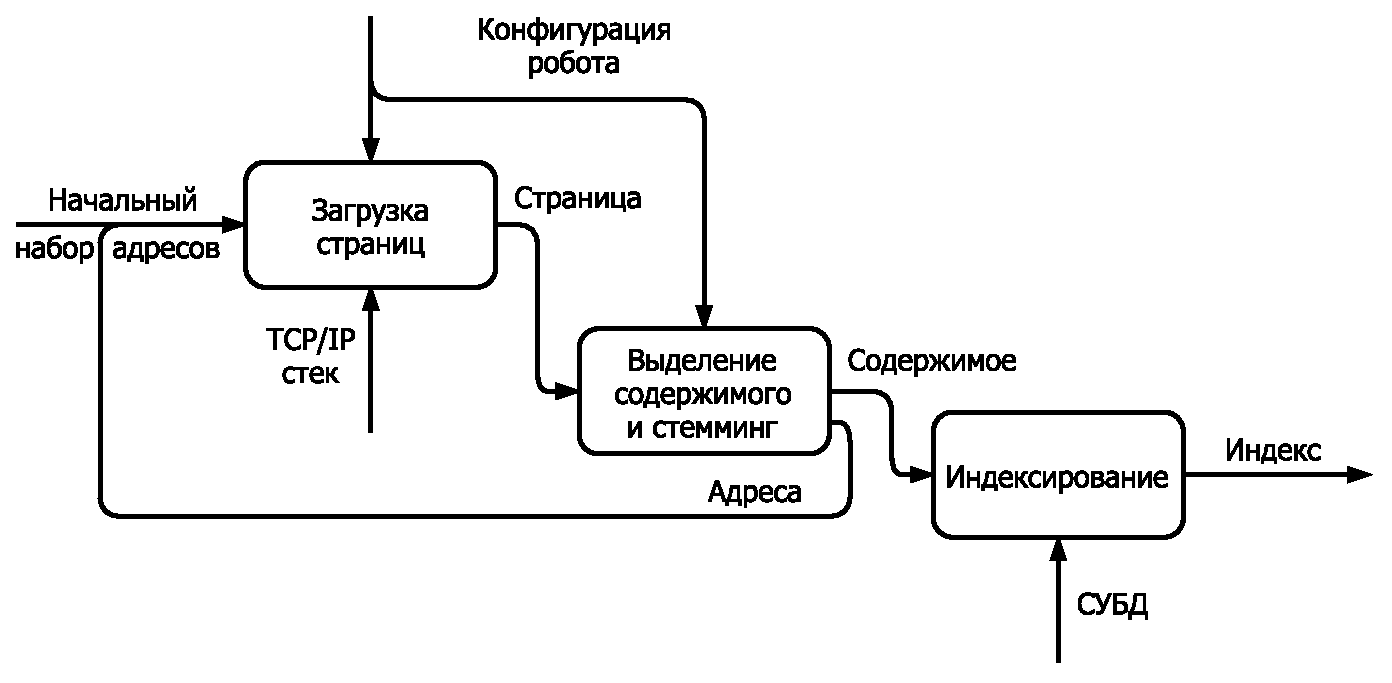
\includegraphics[width=.9\linewidth]{collecting-a1.pdf}
  \caption{IDEF0-A1 поискового робота.}
  \label{fig:collecting-a1}
\end{figure}

Для достижения своей цели поисковому роботу необходимо получить страницу (стек TCP/IP), выделить основное содержимое, разобрать его на слова, выделив основу слова (стемминг), после чего сохранить в БД в форме, удобной для дальнейшего поиска (рис. \ref{fig:collecting-a1}).

Поисковик (рис. \ref{fig:ranking-a0}) по заданному запросу находит все релевантные документы в собранном индексе и возвращает пользователю отсортированный набор документов, соответствующих запросу.

\begin{figure}[h]
  \centering
  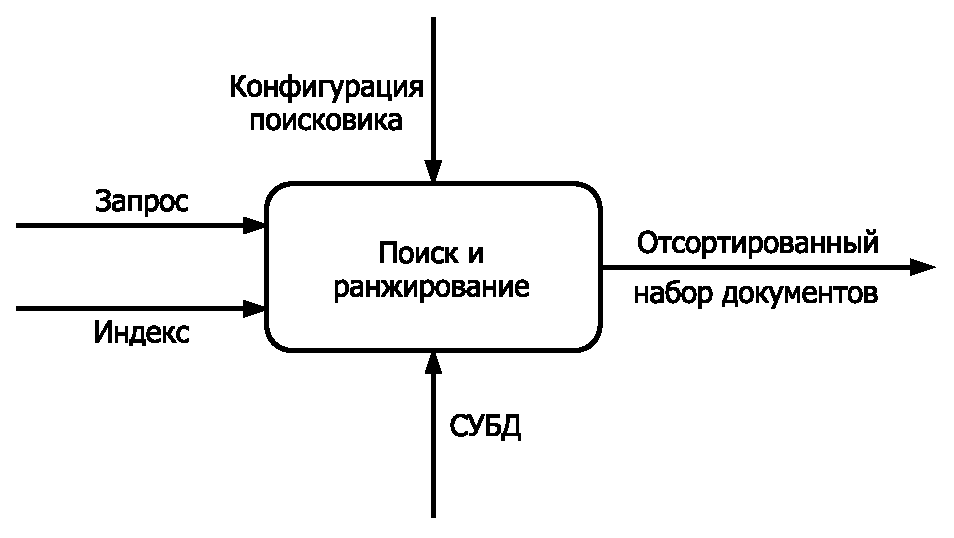
\includegraphics[width=.7\linewidth]{ranking-a0.pdf}
  \caption{IDEF0-A0 поисковика.}
  \label{fig:ranking-a0}
\end{figure}

Поскольку именно поиск документов является главной целью, система должна разрабатываться с учётом тех характеристик документов, которые участвуют в ранжировании, так как от этого зависит способ сбора и хранения данных.

Перед проектированием базы данных необходимо рассмотреть предметную область (рис.~\ref{fig:er}). В целом предметная область определяется через две основные сущности: страницу и слово. Страницы могут ссылаться друг на друга посредством гиперссылок, в тексте которых содержатся определённые слова.

Краткое описание атрибутов:
\begin{enumerate}
  \item URL~--- адрес страницы;
  \item Ключ~--- агрессивно нормализованный адрес URL (см.~\ref{sssec:url-normalization});
  \item PR~--- рейтинг страницы (см.~\ref{sssec:pagerank});
  \item Заголовок~--- совокупность содержимого всех заголовков на странице;
  \item Длина в словах~--- количество слов в странице;
  \item Основа~--- нормализованная форма слова (см.~\ref{sssec:stemming});
  \item Встречаемость~--- количество страниц, включающих данное слово;
  \item IDF~--- производная от встречаемости характеристика (см.~\ref{sssec:tf-idf});
  \item Количество~--- количество определённого слова в странице;
  \item Положение~--- смещение первого вхождения слова (см.~\ref{sssec:position});
  \item TF~--- частота вхождения слова (см.~\ref{sssec:tf-idf});
  \item BM25~--- производная характеристика TF и IDF (см.~\ref{sssec:bm25});
\end{enumerate}

\begin{figure}[h]
  \centering
  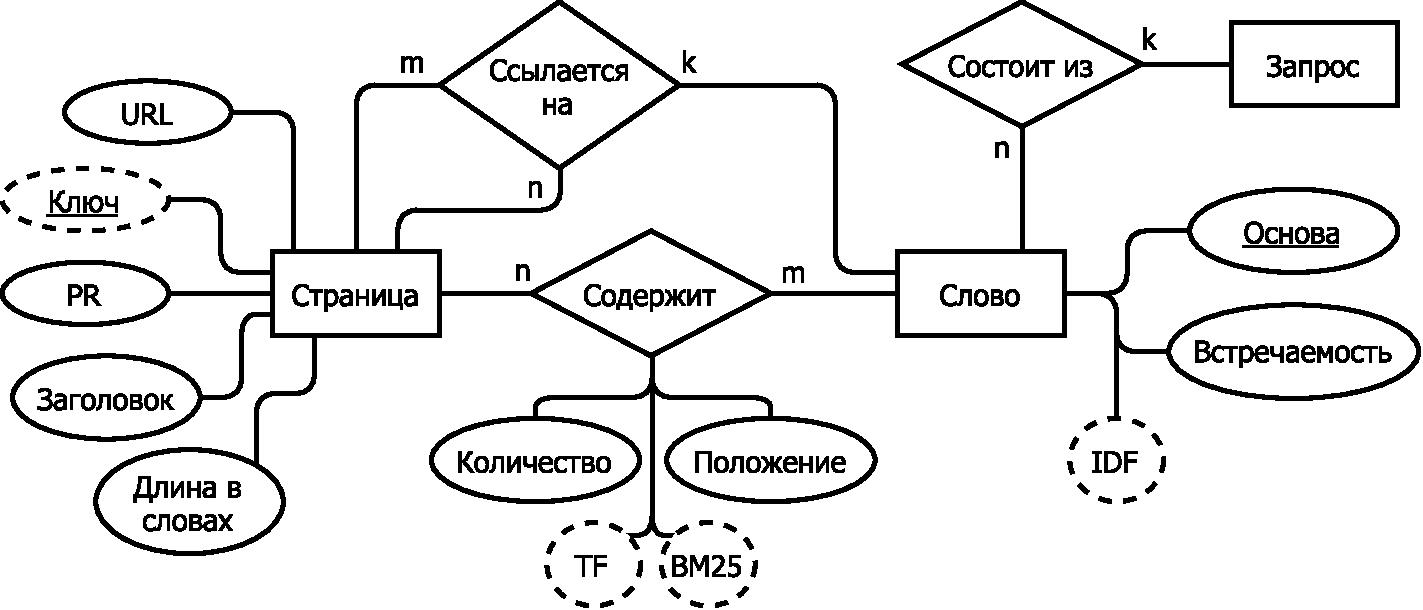
\includegraphics[width=\linewidth]{er.pdf}
  \caption{Концептуальная схема предметной области.}
  \label{fig:er}
\end{figure}

Производные атрибуты (TF, IDF, BM25, ...) рассматриваются далее в этом разделе, как и причины их возникновения.

\section{Ранжирование}
Запрос~--- набор слов с учётом порядка.

Ранжирование~--- упорядочивание документов по принципу наибольшего соответствия запросу.

Фактор (признак)~--- характеристика свойств документа, запроса или их взаимоотношение.

Виды факторов:
\begin{enumerate}
  \item Статические факторы~--- зависящие только от документа;
  \item Факторы, зависящие только от запроса;
  \item Динамические факторы~--- зависящие и от документа, и от запроса.
\end{enumerate}

Функция ранжирования~--- алгоритм, выполняющий ранжирование, используя множество факторов. Такая функция может быть комбинацией других функций ранжирования, используя, например, средневзвешенную сумму или обученную модель регрессии \cite{segaran07}.

Так же факторы условно можно разделить на следующие классы:
\begin{enumerate}
  \item По содержимому: наличие слов из запроса, их частоты, положения;
  \item Ссылочные: популярность страницы, цитируемость;
  \item Метрики, основанные на ответной реакции пользователей.
\end{enumerate}

В данной работе внимание уделено первым двум классам факторов. Класс ответной реакции, функции ранжирования которого часто машинно-обучены, не рассматриваются, так как для получения пригодных результатов требуется достаточно длительное живое обучение, которые в рамках работы не достижимо.


\subsection{Ранжирование по содержимому}
Данный класс основывается на информации, которую можно получить непосредственно из документа:
\begin{itemize}
  \item Общее количество слов в документе (длина документа);
  \item Частота вхождения запрошенных слов в документ;
  \item Положение запрошенных слов в документе;
  \item Расстояние между запрошенными словами в документе;
  \item Входят ли запрошенные слова в заголовки.
\end{itemize}


\subsubsection{TF-IDF} \label{sssec:tf-idf}
Простейшим динамическим фактором является количество вхождения слова $q$ запроса $Q$ ($q\in Q$) в документ $d$: $n_q^d$.

Однако использование данного фактора приводит к тому, что более длинные страницы оказываются более релевантными, даже если относительная доля искомого слова невелика. Поэтому имеет смысл говорить о частоте слова.

Частота слова (от англ. TF~--- term frequency)~--- другой простейший динамический фактор, определяемый как
\begin{equation} \label{eq:tf}
  tf(q, d)=\frac{n_q^d}{|d|}.
\end{equation}

Тогда функция ранжирования на основе только этого фактора примет вид:
\begin{equation}
  score^{tf}(d, Q) = \sum_{q\in Q} tf(q, d).
\end{equation}

Данный фактор позволяет ранжировать страницы исходя из того, сколько раз на ней встретилось искомое слово. Так, выполняя поиск по слову <<python>>, пользователь ожидает увидеть документы, где это слово встречается часто, а не документ о музыканте, который где-то в конце упомянул, что у него дома живёт питон.

Однако данный фактор обладает существенным недостатком: в случае, если в запрос входят популярные (часто встречаемые) слова, то большая часть веса будет приходится именно на них. Для решения этой проблемы вводят обратную частоту документа.

Обратная частота документа (от англ. IDF~--- inverse document frequency)~--- инверсия частоты, с которой слово встречается в документах. Учёт IDF уменьшает вес широкоупотребительных слов.
\begin{equation} \label{eq:idf}
  idf(q)=\log\frac{N}{N_q},
\end{equation}
\begin{conditions}
  $N$ & количество документов в коллекции, $N=|D|$;\\
  $N_q$ & количество документов, содержащих слово $q$, $N_q=|\{d: d\ni q\}|$.
\end{conditions}

Объединяя (\ref{eq:tf}) и (\ref{eq:idf}):
\begin{equation}
  score^{tfidf}(d, Q) = \sum_{q\in Q} tf(q, d) \cdot idf(q, D).
\end{equation}

Теперь вес некоторого слова пропорционален количеству употребления этого слова в документе, и обратно пропорционален частоте употребления слова в других документах коллекции.


\subsubsection{BM25} \label{sssec:bm25}
BM25~--- TF-IDF-подобная функция ранжирования, имеющая лучшую вероятностную интерпретацию \cite{robertson09}:
\begin{equation} \label{eq:bm25}
  score^{bm25}(d, Q) = \sum_{q\in Q}idf(q)\cdot\frac{n_q^d\cdot (k+1)}{n_q^d + k\cdot\left(1-b+b\cdot\frac{|d|}{avg(|d|)}\right)}
\end{equation}
\begin{conditions}
  $k$ и $b$ & свободные коэффициенты, $b\in[0..1]$ и $k \geq 0$;\\
  $avg(|d|)$ & средняя длина документов в коллекции.
\end{conditions}

В данном методе часто используют <<сглаженные>> варианты $idf$, например:
\begin{equation}
  idf(q)=\log\frac{N - N_q + 0.5}{N_q + 0.5}.
\end{equation}

Вышеуказанная формула IDF имеет следующую особенность. Для слов, входящих в более чем половину документов из коллекции, значение IDF отрицательно. Таким образом, при наличии любых двух почти идентичных документов, в одном из которых есть слово, а в другом~--- нет, второй может получить большую оценку. Простейшим решением является игнорирование отрицательных слагаемых в сумме, что эквивалентно игнорированию соответствующих высокочастотных слов:
\begin{equation}
  idf(q)=\max\left(\log\frac{N - N_q + 0.5}{N_q + 0.5}, 0\right).
\end{equation}

Существуют модификации метода, позволяющие уменьшить влияние длины документа для очень больших документов: BM25l \cite{lv11+} и BM25+ \cite{lv11l}, однако в данной работе эта проблема решается восстановлением выбросов (раздел \ref{sssec:outlier}).

Для объединения значений BM25 по разным полям документа (текст, заголовки, входящие ссылки и др.) часто используют различные вариации метода BM25F \cite{robertson09}. Однако в данной работе BM25 является лишь одной из многих частей итоговой функции ранжирования и проблема объединения решена нормализацией каждой части в отдельности (раздел \ref{sssec:normalization}).


\subsubsection{Положение в документе} \label{sssec:position}
Обычно, если страница релевантна поисковому слову, то это слово расположено близко к началу страницы, быть может, даже находится в заголовке. Чтобы воспользоваться этим наблюдением, поисковая система может приписывать результату больший ранг, если поисковое слово встречается в начале документа:
\begin{equation}
  score^{pos}(d, Q)=\sum_{q\in Q}p_q^d,
\end{equation}
где $p_q^d$~--- порядковый номер первого вхождения слова $q$ в документ $d$.


\subsubsection{Расстояние между словами}
Если запрос содержит несколько слов, то часто бывает полезно ранжировать результаты в зависимости от того, насколько близко друг к другу встречаются поисковые слова. Как правило, вводя запрос из нескольких слов, человек хочет найти документы, в которых эти слова концептуально связаны \cite{segaran07}.

\begin{equation}
  score^{dist}(d, Q)=\sum_{\substack{i<j \\ q_i, q_j\in Q}} |p_{q_j}^d - p_{q_i}^d|.
\end{equation}

Эту же функцию ранжирования можно использовать при поиске точного совпадения (фраза, заключённая в кавычки), указав для неё большой вес.

Однако данная функция ранжирования обладает существенным недостатком: это единственная функция из рассмотренных, которая требует хранения в индексе всех вхождений слов в документ, что многократно увеличивает индекс и, как следствие, время запроса. Поэтому в данной работе эта функция не используется.


\subsection{Ссылочное ранжирование}
Все обсуждавшиеся до сих пор функции ранжирования были основаны на содержимом документа. Хотя многие поисковые системы до сих пор работают таким образом, часто результаты можно улучшить, приняв во внимание, что сказано об этом документе в других. Это особенно полезно при индексировании документов сомнительного содержания или таких, которые могли быть созданы спамерами, поскольку маловероятно, что на такие документы ссылаются релевантные.


\subsubsection{Простой подсчёт ссылок}
Простейший способ работы с внешними ссылками заключается в простом подсчёте их количества. Так обычно оцениваются научные работы: считается, что их значимость тем выше, чем чаще их цитируют.

\begin{equation}
  score^{inb}(d) = \big|\{(d_i, d)\in L\}\big|,
\end{equation}
где $L$~--- мн-во всех ссылок $(d_i, d_j)$.

\subsubsection{PageRank} \label{sssec:pagerank}
Этот алгоритм приписывает каждому документу ранг, оценивающий его значимость. Значимость документа вычисляется исходя из значимости ссылающихся на него документов и общего количества ссылок, имеющихся на каждом из них:
\begin{equation} \label{eq:pagerank}
  pr(d) = 0.15 + 0.85 \cdot \left(\sum_{(d_i, d)\in L} \frac{pr(d_i)}{|L_{d_i}|}\right),
\end{equation}
где $L_d$~--- мн-во всех ссылок с документа $d$: $L_d = \{(d, d_j)\in L\}$.

\begin{figure}
  \centering
  \begin{tikzpicture}
    \begin{scope}[every node/.style={circle,thick,draw}]
      \node (A) at (-1.5,0) {$A (0.8)$};
      \node (B) at (1,3.5) {$B (0.42)$};
      \node (C) at (2.5,1) {$C (?)$};
      \node (E) at (2.5,-3.5) {$E (0.6)$};
      \node (F) at (6,3) {$F (0.9)$};
    \end{scope}

    \begin{scope}[>={Stealth[black]},
      every node/.style={fill=white,circle},
      every edge/.style={draw=red,very thick}]
      \path[->] (A) edge node {$0.2$} (C);
      \path[->] (E) edge node {$0.3$} (C);
      \path[->] (F) edge node {$0.3$} (C);
      \path[->] (A) edge (B);
      \path[->] (A) edge (E);
      \path[->] (B) edge (F);
      \path[->] (E) edge (F);
      \path[->] (F) edge[bend left=40] (E);
      \path[<-] (E) edge ++(-2,0);
      \path[->] (A) edge ++(0,-2);
      \path[<-] (A) edge ++(-2.3,0);
      \path[->] (F) edge ++(2,0);
      \path[<-] (F) edge ++(0,2);
      \path[<-] (B) edge ++(-3,0);
    \end{scope}
  \end{tikzpicture}
  \caption{Вычисление ранга PageRank документа $C$.}
  \label{fig:pagerank}
\end{figure}

Например, PageRank страницы $C$ (рис. \ref{fig:pagerank}) вычисляется как
\begin{equation}
  \begin{split}
    pr(C) &= 0.15 + 0.85\cdot\left(\frac{pr(A)}{|L_A|}+\frac{pr(F)}{|L_F|}+\frac{pr(E)}{|L_E|}\right)\\
    &= 0.15 + 0.85\cdot\left(\frac{0.8}{4}+\frac{0.9}{3}+\frac{0.6}{2}\right)\\
    &= 0.15 + 0.85\cdot 0.8 = 0.83.
  \end{split}
\end{equation}

Увы, имеется небольшая ловушка~--- в данном примере для всех документов, ссылающихся на $C$, уже вычислен ранг, что является тривиальным случаем. Необходимо вычислить ранги для множества документов, ранги которых ещё не известны.

Решение состоит в том, чтобы присвоить всем документам произвольный начальный ранг (отличный от нуля, например 1) и провести несколько итераций. Количество необходимых итераций зависит от числа страниц и в нашем случае (количество страниц до миллиона) 20-30 должно быть достаточно. Google, например, просчитывает ранги для своего индекса приблизительно за 100 итераций.

Функция ранжирования в данном случае предельно проста:
\begin{equation}
  score^{pr}(d) = pr(d).
\end{equation}


\subsubsection{Использование текста ссылки}
Ещё один полезный способ ранжирования результатов~--- использование текста ссылок на документ при определении степени её релевантности запросу. Часто удаётся получить более качественную информацию из того, что сказано в ссылках, ведущих на документ, чем из самого документа.

Таким образом, учитывается ранг источников тех ссылок, которые ведут на оцениваемую страницу и содержат слова из запроса:
\begin{equation}
  score^{link}(d, Q) = \sum_{\substack{(d_i, d, t)\in L \\ q\in Q\cap t}} pr(d_i),
\end{equation}
где $t$ в $(d_i, d, t)$~--- текст ссылки $(d_i, d)$.


\subsection{Объединение функций ранжирования}
Теперь, имея все необходимые функции ранжирования, необходимо получить итоговую функцию, которая будет являться средневзвешенной суммой нормализованных функций ранжирования.


\subsubsection{Нормализация} \label{sssec:normalization}
Чтобы сравнивать результаты, получаемые различными функциями ранжирования, необходимо как-то нормализовать их, то есть привести к одному и тому же диапазону и направлению: от $0$ (наихудший результат) до $1$ (наилучший результат):
\begin{equation} \label{eq:simple-norm}
  norm(s, s_{min}, s_{max}) = \begin{cases}
    \frac{s-s_{min}}{s_{max} - s_{min}}, \; s_{max} > s_{min}\\
    1, \; \text{иначе}
  \end{cases},
\end{equation}
где $s$~--- результат функции ранжирования.

В случае, когда $s_{min}=s_{max}$, то есть значение функции для всех документов одинаково, будем считать, что все документы получили максимальную оценку.


\subsubsection{Обработка выбросов} \label{sssec:outlier}
Выброс~--- результат измерения, выделяющийся из общей выборки. Например, среди документов, полученных по запросу <<ecmascript>>, встречается спецификация, а так как ссылок, включающих искомое слово, на неё ведёт много, то и $score^{link}$ для данного документа будет сильно выше других документов. Это приведёт к дискредитации $score^{link}$~--- остальные документы будут иметь низкие показатели. Таким образом, необходимо ввести определённый верхний (нижний) порог, выше (ниже) которого функция обращается в $1$ ($0$).

Простейший метод определения выброса основан на межквартильном расстоянии: выбросами считается всё, что не попадает в диапазон
\begin{equation}
  \left[(s_{25}-1.5\cdot (s_{75}-s_{25})), (s_{75}+1.5\cdot (s_{75}-s_{25}))\right],
\end{equation}
\begin{conditions}
  $s_{25}$ & 0.25-квантиль;\\
  $s_{75}$ & 0.75-квантиль.
\end{conditions}

Однако использование такого критерия приводит к тому, что по некоторым функциям ранжирования $0$ или $1$ не достижимы (максимум или минимум внутри диапазона). Поэтому имеет смысл в качестве диапазона брать $[s_{min}', s_{max}']$, где
\begin{equation}
  \begin{split}
    s_{min}'&=\max(s_{min}, s_{25}-1.5\cdot (s_{75}-s_{25})),\\
    s_{max}'&=\min(s_{max}, s_{75}+1.5\cdot (s_{75}-s_{25})).
  \end{split}
\end{equation}


\subsubsection{Итоговая функция ранжирования}
Теперь, если функцию нормировки (\ref{eq:simple-norm}) переписать как
\begin{equation}
  norm(s) = \begin{cases}
    1, \; (s > s_{max}')\lor (s_{max}' = s_{min}')\\
    0, \; s < s_{min}'\\
    \frac{s-s_{min}'}{s_{max}' - s_{min}'}, \text{иначе}
  \end{cases},
\end{equation}
то итоговую формулу для функции ранжирования можно задать как средневзвешенную сумму всех нормализованных функций:
\begin{equation}
  score(d, Q)=\frac{\sum w_s\cdot norm(score^s(d, Q))}{\sum w_s}.
\end{equation}

\section{Сбор информации}
Сбор информации является важной задачей в системах полнотекстового поиска, потому что именно качество собранной информации главным образом влияет на репрезентативность выборки, которую получит пользователь системы, совершающий запрос.

Данная задача порождает множество проблем, таких как: огромное количество заведомо нерелевантных страниц, ограничительная пропускная способность каналов, слабость серверов и пр.

В данном разделе приводится описание возникающих проблем и способы борьбы с ними.


\subsection{Фильтрация посещённых страниц}
Во время обхода важно отбрасывать ссылки, ведущие на страницы, которые уже были посещены или находятся в очереди на обработку. Очевидное на первый взгляд решение проблемы~--- использование ассоциативных массивов (причём скорее всего именно хеш-таблиц)~--- довольно требовательно к памяти.

Поэтому для фильтрации посещённых страниц применяется фильтр Блума.


\subsubsection{Фильтр Блума}
Фильтр Блума~--- вероятностная структура данных, позволяющая компактно хранить множество элементов и проверять принадлежность заданного элемента к множеству. При этом существует вероятность получить ложноположительный результат, то есть ситуацию, когда элемента в множестве нет, но фильтр сообщает, что элемент есть.

Фильтр Блума может использовать любой объём памяти, заранее заданный пользователем, причём чем он больше, тем меньше вероятность ложного срабатывания. Поддерживается операция добавления новых элементов в множество, но не удаления существующих (если только не используется модификация со счётчиками).

\begin{figure}[h]
  \centering
  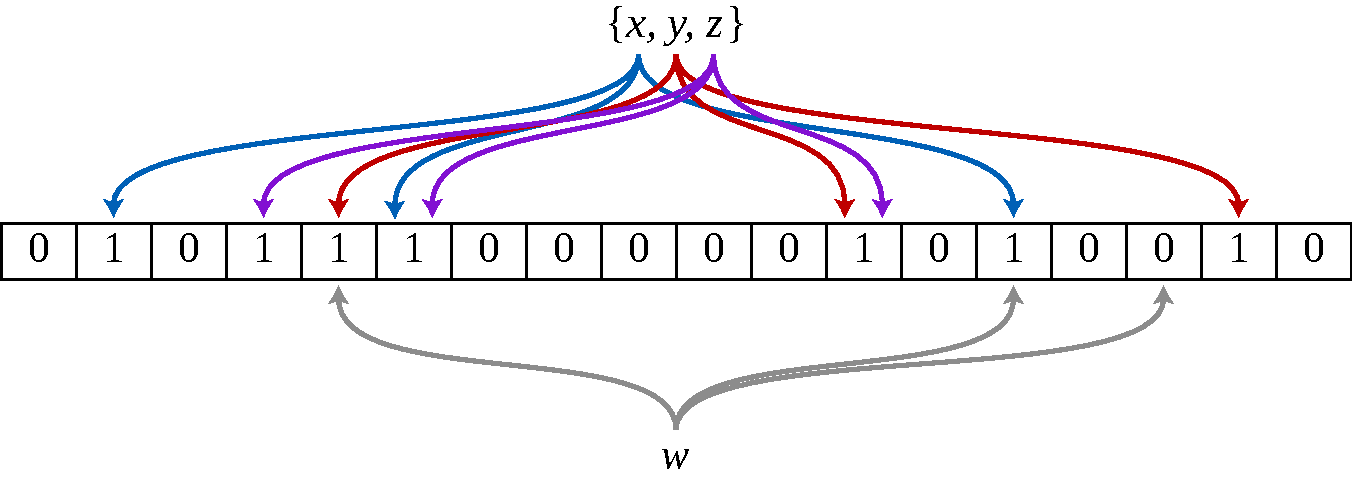
\includegraphics[width=\textwidth]{bloom-filter.pdf}
  \caption{Пример фильтра Блума с $m=18$ и $k=3$.}
\end{figure}

Фильтр Блума представляет собой битовый массив из $m$ бит. Изначально, когда структура данных хранит пустое множество, все $m$ бит обнулены. Пользователь должен определить $k$ независимых хеш-функций $h_i$, отображающих каждый элемент в одну из $m$ позиций битового массива достаточно равномерным образом.

Для добавления элемента $e$ необходимо записать единицы на каждую из позиций $h_i(e)$ битового массива.

Для проверки принадлежности элемента $e$ к множеству хранимых элементов, необходимо проверить состояние битов $h_i$. Если хотя бы один из них равен нулю, элемент не может принадлежать множеству (иначе бы при его добавлении все эти биты были установлены). Если все они равны единице, то структура данных сообщает, что $e$ принадлежит множеству. При этом может возникнуть две ситуации: либо элемент действительно принадлежит к множеству, либо все эти биты оказались установлены по случайности при добавлении других элементов, что и является источником ложных срабатываний в этой структуре данных.

Согласно \cite{broder02}, для заданных $n$~--- числа ожидаемых элементов в множестве и $p$~--- максимальной вероятности ложноположительного срабатывания возможно вычислить оптимальный размер $m$ как
\begin{equation}
  m=-\frac{n\ln p}{(\ln 2)^2},
\end{equation}
и оптимальное количество хеш-функций как
\begin{equation}
  k=\frac{m}{n}\ln 2.
\end{equation}


\subsubsection{Параметры фильтра Блума}
Количество максимально ожидаемых страниц очевидным образом зависит от глубины обхода:
\begin{equation}
  n=l^{d-1},
\end{equation}
\begin{conditions}
  $d$ & максимальная глубина обхода;\\
  $l$ & среднее количество ссылок на странице.
\end{conditions}

Так, при $l=100$, $d=4$ и $p=0.00001$ (ожидается не более одного ложноположительного срабатывания на 10 миллионов) потребуется всего $\approx 2.86$МБ данных.


\subsection{Стандарт исключений для роботов} \label{ssec:robotstxt}
Когда владельцы сайта хотят ограничить доступ к определённым страницам для поисковых ботов, они используют для этого файл \verb|robots.txt|, находящийся в корне сайта (то есть по пути \verb|/robots.txt|). Это может быть полезно для ограничения частоты запросов со стороны роботов, запрета индексирования динамический и служебных страниц.

Формат файла имеет следующий вид:
\begin{verbatim}
<поле>:<необязательный пробел><значение><необязательный пробел>
\end{verbatim}

Стоит заметить, что вместо пробела могут использоваться также другие пробельные символы, а \verb|поле| является регистронезависимым.

Основные используемые поля:
\begin{itemize}
  \item \verb|user-agent|: стандартное поле, используется для задания имени бота, которому адресованы последующие правила, либо \verb|*|, если всем;
  \item \verb|disallow|: стандартное поле, используется для задания пути, индексация которого запрещена. В пути разрешены два спец-символа: \verb|*| (любое количество любых символов) и \verb|$| (конец пути). Причём путь, к примеру, \verb|/path/to/file| действует аналогично \verb|/path/to/file*|;
  \item \verb|crawl-delay|: нестандартное поле, используется для задания минимальной задержки в секундах между запросами со стороны робота.
\end{itemize}


\subsection{Разбор страницы}
После загрузки страницы необходимо подготовить её к индексации~--- выделить полезную информацию: определить заголовок, слова для индексации, ссылки для загрузки.


\subsubsection{Декодирование мнемоник HTML}
Мнемоника~--- это конструкция SGML, которая ссылается на символ из набора символов текстового файла. В HTML предопределено большое количество спецсимволов. Чтобы вставить определённый символ в разметку, нужно вставить определенную ссылку-мнемонику в HTML-структуру.

Мнемоника имеет вид \verb|&...;|. Так, например, буква <<q>> может представляться как \verb|&#113;|, а <<--->> как \verb|&mdash;|.

Необходимость в декодировании символов-мнемоник исходит из нескольких причин:
\begin{enumerate}
  \item Мнемоники встречаются в заголовках страницы, который будет отображаться пользователю при поиске;
  \item Должны индексироваться не мнемоники, а только их значения. Так, мнемоника \verb|&empty;| (<<$\varnothing$>>) не должна индексироваться как слово <<empty>>.
\end{enumerate}


\subsubsection{Выделение содержимого} \label{sssec:readability}
Далеко не вся информация на странице ценна для поиска. Например, информация, размещённая в подвале и по сторонам страницы несёт обычно служебную информацию, которая может быть полезна при обходе страниц (так как может содержать полезные ссылки), но бесполезна конечному пользователю. Поэтому ставится вопрос об ограничении индексации исключительно полезными частями страницы. Для этого необходимы методы выделения такой информации, которые в основном базируются на эвристики и неплохо работают во многих случаях \cite{pomikalek11}.

Для получения основного содержимого во многих случаях достаточно сохранять только текстовые элементы HTML, то есть блоки текста, которые не прерывались разметкой, которые имеют более чем десяток слов. Люди выбирают один из двух типов текста для двух различных мотивов написания текста: <<навигационного>> и <<информационного>>.

Для элементов навигации обычно применяется текст, состоящий из нескольких слов (например, <<STOP>>, <<Прочтите это>>, <<Нажмите здесь>>), в то время как для основого содержимого используется много слов.

В то время как это разделение работает во множестве случаев, все становится сложнее с заголовками, короткими предложениями, отказами от ответственности, авторскими правами и другими колонтитулами.

Есть более сложные стратегии, а также функции, которые помогают отделять основное содержание от шаблонного \cite{kohlschutter10}:
\begin{enumerate}
  \item Рассмотренная выше плотность HTML-тегов;
  \item Ссылочная плотность (количество слов внутри ссылок по сравнению с общим количеством слов в блоке);
  \item Связь текущего блока с контекстом (с предыдущими и следующими блоками);
  \item DOM-структура документа (\verb|<article>|, \verb|<section>| и другие);
  \item Визуальное изображение страницы (например, большие изображения, окружённые текстом);
  \item Различные машинно-обученные алгоритмы.
\end{enumerate}

Результирующий алгоритм, используя комбинацию этих факторов, рекурсивно оценивает все узлы документа, находя наиболее похожие на основное содержимое.


\subsubsection{Выделение ссылок} \label{sssec:links}
Ссылки на странице могут быть обнаружены во многих местах: \verb|<a>|, \verb|<link>|, \verb|<script>| и др. Но для поискового бота по (x)html интерес представляют только ссылки в \verb|<a>|, причём далеко не все. Для уменьшения количества бесполезных запросов, связанных, например, с неиспользуемым языком, которые скорее всего всё равно будут выявлены на этапе получения заголовков (HTTP-заголовок \verb|content-language|), можно попробовать угадать по адресу ссылки релевантность.

Рассмотрим несколько методов фильтрации ссылок:
\begin{enumerate}
  \item По наличию букв из неиспользуемых алфавитов в пути ссылки. Действительно, если ссылка содержит несколько таких символов, то скорее всего представленная информация на странице имеет тот же язык;
  \item Использование чёрного или белого списков расширений, которые позволяет откидывать страницы с заведомо нерелевантной информацией, например \verb|.jpg|. Чёрный список задаётся списком запрещённых разрешений, в том время как белый список~--- разрешённых, например \verb|.html|, \verb|.asp| и \verb|.php|;
  \item Фильтрация доменов, так же основанная на чёрном или белом списках;
  \item Фильтрация поддоменов, основанная на некоторой эвристике. Например, поддомены \verb|git.| и \verb|svn.| часто содержат соответствующие репозитории, индексировать которые в большинстве случаев не имеет смысла.
\end{enumerate}


Кроме того, ссылки, заданные через \verb|<a>| могут иметь атрибут \verb|rel="nofollow"|, который используется для того, чтобы запретить учитывать данную ссылку поисковыми ботами при индексации страницы и передавать по ней вес данной страницы при расчёте PageRank. Чаще всего таким образом помечаются рекламные ссылки. Несмотря на то, что в индекс данные ссылки не попадают, включать их в оборот всё же имеет смысл.


\subsubsection{Стоп-слова}
Существование заведомо высокочастотных слов (таких как <<an>>, <<and>>, <<и>>, <<как>> и др.) ведёт к раздуванию индекса и, как следствие, замедлению работы поиска. При этом их вклад в ранжирование минимален. Поэтому разумно отказаться от индексирования таких слов вообще, путём занесения их в списки так называемых стоп-слов.


\subsubsection{Стемминг} \label{sssec:stemming}
Стемминг~---процесс нормализации слов путём выделения основы. Это позволяет учитывать морфологически близкие слова как формы одно и того же слова (например, <<connect>> и <<connected>> или <<чистый>> и <<чистая>>), что сильно улучшает ранжирование и упрощает поиск.

Наиболее известен алгоритм стемминга Портера. Алгоритм не использует баз основ слов, а работает, последовательно применяя ряд правил отсечения окончаний и суффиксов \cite{porter97}.

Рассмотрим версию алгоритма для русского языка \cite{porter06}.

Во-первых, в слове выделяются три зоны:
\begin{description}
  \item[RV] область слова после первой гласной. Может быть пустой, если гласных в слове нет;
  \item[R1] область слова после первого сочетания <<гласная-согласная>>;
  \item[R2] область R1 после первого сочетания <<гласная-согласная>>.
\end{description}

Далее выделяются группы окончаний слов:
\begin{itemize}
  \item Совершенного герундия (<<в>>, <<вши>>, <<вшись>> после <<а>> или <<я>>; <<ив>>, <<ивши>>, <<ившись>>, <<ыв>>, <<ывши>>, <<ывшись>>);
  \item Прилагательных (<<ее>>, <<ие>>, <<ые>>, <<ое>>, <<ими>>, <<ыми>>, <<ей>>, <<ий>>, <<ый>>, <<ой>>, <<ем>>, <<им>>, <<ым>>, <<ом>>, <<его>>, <<ого>>, <<ему>>, <<ому>>, <<их>>, <<ых>>, <<ую>>, <<юю>>, <<ая>>, <<яя>>, <<ою>>, <<ею>>);
  \item Причастных (<<eм>>, <<нн>>, <<вш>>, <<ющ>>, <<щ>> после а и я; <<ивш>>, <<ывш>>, <<ующ>>);
  \item Возвратных (<<ся>>, <<сь>>);
  \item Глагольных (<<ла>>, <<на>>, <<ете>>, <<йте>>, <<ли>>, <<й>>, <<л>>, <<ем>>, <<н>>, <<ло>>, <<но>>, <<ет>>, <<ют>>, <<ны>>, <<ть>>, <<ешь>>, <<нно>> после а или я; <<ила>>, <<ыла>>, <<ена>>, <<ейте>>, <<уйте>>, <<ите>>, <<или>>, <<ыли>>, <<ей>>, <<уй>>, <<ил>>, <<ыл>>, <<им>>, <<ым>>, <<ен>>, <<ило>>, <<ыло>>, <<ено>>, <<ят>>, <<ует>>, <<уют>>, <<ит>>, <<ыт>>, <<ены>>, <<ить>>, <<ыть>>, <<ишь>>, <<ую>>, <<ю>>);
  \item Существительных (<<а>>, <<ев>>, <<ов>>, <<ие>>, <<ье>>, <<е>>, <<иями>>, <<ями>>, <<ами>>, <<еи>>, <<ии>>, <<и>>, <<ией>>, <<ей>>, <<ой>>, <<ий>>, <<й>>, <<иям>>, <<ям>>, <<ием>>, <<ем>>, <<ам>>, <<ом>>, <<о>>, <<у>>, <<ах>>, <<иях>>, <<ях>>, <<ы>>, <<ь>>, <<ию>>, <<ью>>, <<ю>>, <<ия>>, <<ья>>, <<я>>);
  \item Превосходных (<<ейш>>, <<ейше>>);
  \item Словообразовательных (<<ост>>, <<ость>>);
  \item Адъективированных (определяется как прилагательное или причастие + прилагательное окончание).
\end{itemize}

При поиске окончания из всех возможных выбирается наиболее длинное. Например, в слове <<величие>> выбираем окончание <<ие>>, а не <<е>>.

Все проверки производятся над областью RV. Так, при проверке на совершенный герундий предшествующие буквы <<а>> и <<я>> также должны быть внутри RV. Буквы перед RV не участвуют в проверках вообще.

\begin{enumerate}
  \item Найти окончание совершенного герундия. Если оно существует~--- удалить его и завершить этот шаг. Иначе, удаляем возвратное окончание, если существует. Затем по порядку удаляется адъективированное окончание, глагольное окончание, окончание существительного. Как только одно из них найдено~--- шаг завершается;
  \item Если слово оканчивается на <<и>>~--- удалить <<и>>;
  \item Если в R2 найдётся словообразоваельное окончание~--- удалить его.
  \item Возможен один из трёх вариантов:
    \begin{enumerate}
      \item Если слово оканчивается на <<нн>>~--- удалить последнюю букву;
      \item Если слово оканчивается на превосходное окончание~--- удаляем его и снова проверяем <<нн>>;
      \item Если слово оканчивается на <<ь>>~--- удалить его.
    \end{enumerate}
\end{enumerate}

Аналогично существуют версии алгоритма для многих европейских языков, однако в данной работе используется только русский и английский языки.


\subsubsection{URL нормализация} \label{sssec:url-normalization}
Различные URL могут указывать на одну и ту же страницу, но отличаться при этом незначительно.

URL нормализация~--- процесс приведения URL к каноничному виду, путём применения различных правил трансляции адресов. Не все правила дают строго эквивалентные URL, однако на практике эти эвристики работают неплохо \cite{pant04}.

Ключ страницы~--- своего рода хеш, получаемый в результате агрессивной нормализации, то есть применения всех правил, указанных в данном разделе.

Относительно безопасные преобразования:
\begin{enumerate}
  \item Конвертация в нижний регистр компонентов схемы и хоста: \\ \verb|HTTP://www.Example.com/| в \verb|http://www.example.com/|;
  \item Удаление относительных каталогов, сегментов-точек: \\ \verb|http://example.com/../a/b/../c/./d| в \verb|http://example.com/a/c/d|;
  \item Удаление фрагментов: \\ \verb|http://example.com/bar.html#section1| в \verb|http://example.com/bar.html|;
  \item Удаление конечного слеша: \\ \verb|http://example.com/foo/| в \verb|https://example.com/foo|;
  \item Удаление порта по умолчанию: 80 для http и 443 для https \\ \verb|http://example.com:80| в \verb|http://example.com|;
  \item Перевод IDN в unicode: \\ \verb|http://xn--e1afmkfd.xn--80akhbyknj4f/| в \verb|http://пример.испытание/|.
\end{enumerate}

Преобразования, которые можно использовать для проверки эквивалентности двух страниц, но не при запросе:
\begin{enumerate}
  \item Удаление головного индекса (\verb|index.html|, \verb|default.aspx| и другие): \\ \verb|http://example.com/index.html| в \verb|http://www.example.com/|;
  \item Удаление дублированных слешей: \\ \verb|http://example.com/foo//bar.html| в \verb|http://example.com/foo/bar.html|;
  \item Удаление \verb|www.|: \\ \verb|http://www.example.com/| в \verb|http://example.com/|;
  \item Сокращение идентификаторов протокола: \\ \verb|https://example.com| в \verb|http://example.com|;
  \item Конвертация в нижний регистр всего URL: \\ \verb|HTTP://example.COM/TEST.html| в \verb|http://example.com/test.html|;
\end{enumerate}

Кроме того, так как для работы с динамическими страницами (их URL чаще всего содержат поисковую компоненту) требуется наличие отлаженного и надёжного метода определения дубликатов страницы, в данной работе было решено отказаться от подобных ссылок~--- к ссылке добавляется атрибут \verb|rel="nofollow"|, а запрос отбрасывается: \\ \verb|http://example.com/?id=123&q=test| в \verb|http://example.com/|.

